% Options for packages loaded elsewhere
\PassOptionsToPackage{unicode}{hyperref}
\PassOptionsToPackage{hyphens}{url}
%
\documentclass[
]{book}
\usepackage{amsmath,amssymb}
\usepackage{lmodern}
\usepackage{iftex}
\ifPDFTeX
  \usepackage[T1]{fontenc}
  \usepackage[utf8]{inputenc}
  \usepackage{textcomp} % provide euro and other symbols
\else % if luatex or xetex
  \usepackage{unicode-math}
  \defaultfontfeatures{Scale=MatchLowercase}
  \defaultfontfeatures[\rmfamily]{Ligatures=TeX,Scale=1}
\fi
% Use upquote if available, for straight quotes in verbatim environments
\IfFileExists{upquote.sty}{\usepackage{upquote}}{}
\IfFileExists{microtype.sty}{% use microtype if available
  \usepackage[]{microtype}
  \UseMicrotypeSet[protrusion]{basicmath} % disable protrusion for tt fonts
}{}
\makeatletter
\@ifundefined{KOMAClassName}{% if non-KOMA class
  \IfFileExists{parskip.sty}{%
    \usepackage{parskip}
  }{% else
    \setlength{\parindent}{0pt}
    \setlength{\parskip}{6pt plus 2pt minus 1pt}}
}{% if KOMA class
  \KOMAoptions{parskip=half}}
\makeatother
\usepackage{xcolor}
\IfFileExists{xurl.sty}{\usepackage{xurl}}{} % add URL line breaks if available
\IfFileExists{bookmark.sty}{\usepackage{bookmark}}{\usepackage{hyperref}}
\hypersetup{
  pdftitle={마케팅/고객 분석 그룹스터디},
  pdfauthor={Chad (Chungil Chae)},
  hidelinks,
  pdfcreator={LaTeX via pandoc}}
\urlstyle{same} % disable monospaced font for URLs
\usepackage{longtable,booktabs,array}
\usepackage{calc} % for calculating minipage widths
% Correct order of tables after \paragraph or \subparagraph
\usepackage{etoolbox}
\makeatletter
\patchcmd\longtable{\par}{\if@noskipsec\mbox{}\fi\par}{}{}
\makeatother
% Allow footnotes in longtable head/foot
\IfFileExists{footnotehyper.sty}{\usepackage{footnotehyper}}{\usepackage{footnote}}
\makesavenoteenv{longtable}
\usepackage{graphicx}
\makeatletter
\def\maxwidth{\ifdim\Gin@nat@width>\linewidth\linewidth\else\Gin@nat@width\fi}
\def\maxheight{\ifdim\Gin@nat@height>\textheight\textheight\else\Gin@nat@height\fi}
\makeatother
% Scale images if necessary, so that they will not overflow the page
% margins by default, and it is still possible to overwrite the defaults
% using explicit options in \includegraphics[width, height, ...]{}
\setkeys{Gin}{width=\maxwidth,height=\maxheight,keepaspectratio}
% Set default figure placement to htbp
\makeatletter
\def\fps@figure{htbp}
\makeatother
\setlength{\emergencystretch}{3em} % prevent overfull lines
\providecommand{\tightlist}{%
  \setlength{\itemsep}{0pt}\setlength{\parskip}{0pt}}
\setcounter{secnumdepth}{5}
\usepackage{kotex}
\usepackage{booktabs}
\usepackage{kotex}
\ifLuaTeX
  \usepackage{selnolig}  % disable illegal ligatures
\fi
\usepackage[]{biblatex}
\addbibresource{book.bib}
\addbibresource{packages.bib}

\title{마케팅/고객 분석 그룹스터디}
\author{Chad (Chungil Chae)}
\date{2022-01-15}

\begin{document}
\maketitle

{
\setcounter{tocdepth}{1}
\tableofcontents
}
\hypertarget{uxc2a4uxd130uxb514-uxae30uxbcf8uxc815uxbcf4}{%
\chapter{스터디 기본정보}\label{uxc2a4uxd130uxb514-uxae30uxbcf8uxc815uxbcf4}}

\hypertarget{uxbbf8uxd305-uxc2dcuxac04uxacfc-uxb0a0uxc790-uxbc0f-uxc7a5uxc18c}{%
\section{미팅 시간과 날자 및 장소}\label{uxbbf8uxd305-uxc2dcuxac04uxacfc-uxb0a0uxc790-uxbc0f-uxc7a5uxc18c}}

\begin{itemize}
\tightlist
\item
  스터디 기간:

  \begin{itemize}
  \tightlist
  \item
    2022년 1월 08일 (SA) - 2022년 3월 12일 (SA)
  \end{itemize}
\item
  스터디 시간

  \begin{itemize}
  \tightlist
  \item
    오전 10시(한국시간) 시작
  \item
    오전 11:30 (room closing at 11:45 am) 종료
  \end{itemize}
\item
  Zoom URL

  \begin{itemize}
  \tightlist
  \item
    \url{https://tamuc.zoom.us/j/94691565814?pwd=WmtsYyt3c1BSQmJ0bHdCQS9MRGVyQT09} (권한가진(참가자)들만 억세스 가능)
  \item
    Meeting ID: 946 9156 5814
  \end{itemize}
\item
  스터디 목적:

  \begin{itemize}
  \tightlist
  \item
    마케팅 컨텍스트에서 데이터분석과 고객분석의 기초 분석 능력향상
  \end{itemize}
\item
  세션 포멧:

  \begin{itemize}
  \tightlist
  \item
    30 분 (max) 발표 (챕터 서머리)
  \item
    45\textasciitilde50분간 이어지는 논의/토론 (examples, application, needs, etc). - 스터디 관련자료
  \item
    \url{https://drive.google.com/drive/folders/1dyCazsp8dICExaByzMfAyrkwrDO546Zf?usp=sharing} (권한가진(참가자)들만 억세스 가능)
  \end{itemize}
\item
  공유폴더

  \begin{itemize}
  \tightlist
  \item
    \url{https://drive.google.com/drive/folders/1dyCazsp8dICExaByzMfAyrkwrDO546Zf?usp=sharing} (권한가진(참가자)들만 억세스 가능)
  \end{itemize}
\end{itemize}

\hypertarget{uxba64uxbc84}{%
\section{멤버}\label{uxba64uxbc84}}

\hypertarget{facilitators}{%
\subsection{Facilitators}\label{facilitators}}

\begin{itemize}
\tightlist
\item
  윤승원 Texas A\&M University-Commerce 고등교육/교육공학 박사과정 주임교수 1.217.493.5741 \href{mailto:hrdswon@gmail.com}{\nolinkurl{hrdswon@gmail.com}} (R에 익숙. Python도 책 5권정도 공부했지만 자주 사용하지는 않음)
\item
  채충일 Kean Univ. Wenzou 경영대 비지니스 애널리틱스 조교수 86-133-2598-0138 \href{mailto:chadchae@gmail.com}{\nolinkurl{chadchae@gmail.com}}
\end{itemize}

\hypertarget{participants}{%
\subsection{Participants}\label{participants}}

각 현업의 실무 또는 경영진 8분

\hypertarget{uxad50uxc7ac}{%
\section{교재}\label{uxad50uxc7ac}}

\begin{itemize}
\tightlist
\item
  R For Marketing Research and Analytics (Use R!) 2nd ed \autocite{chapman2015r}

  \begin{itemize}
  \tightlist
  \item
    \url{https://www.amazon.com/Marketing-Research-Analytics-Use-dp-3030143155/dp/3030143155/ref=dp_ob_title_bk}
  \end{itemize}
\item
  Python for Marketing Research and Analytics 1st ed.~2020 \autocite{schwarz2020python}

  \begin{itemize}
  \tightlist
  \item
    \url{https://www.amazon.com/Python-Marketing-Research-Analytics-Schwarz/dp/3030497194/ref=sr_1_3?crid=K9T2N4ZKQ4QD\&keywords=Python+for+Marketing+Research+and+Analytics\&qid=1641325026\&s=books\&sprefix=python+for+marketing+research+and+analytics\%2Cstripbooks\%2C243\&sr=1-3}
  \end{itemize}
\end{itemize}

\hypertarget{uxc2a4uxcf00uxc974}{%
\section{스케쥴}\label{uxc2a4uxcf00uxc974}}

\begin{itemize}
\tightlist
\item
  스터디의 원활한 진행을 위해 관심있는 발표를 진행할 관심있는 챕터와 스케쥴을 선정해 주세요:
\item
  Week 1 (Jan 08) : \textbf{Yoon \& Chae}

  \begin{itemize}
  \tightlist
  \item
    Overview of R, Expectations
  \item
    (pp.~50, Chs 1 \& 2, )
  \end{itemize}
\item
  Week 2 (Jan 15) : \textbf{손경희}

  \begin{itemize}
  \tightlist
  \item
    Describing Data \& Continuous Vars
  \item
    (pp.~56, Chs 3\&4)
  \end{itemize}
\item
  Week 3 (Jan 22) : \textbf{윤승원}

  \begin{itemize}
  \tightlist
  \item
    Comparing Groups \& Tests
  \item
    (pp.~40, Chs 5\&6)
  \end{itemize}
\item
  \textbf{Week 4 (Jan 29) :No meeting, New Year Celebration}
\item
  Week 5 (Feb 05) : \textbf{이진재}

  \begin{itemize}
  \tightlist
  \item
    Linear Models \& Complexity (PCA)
  \item
    (pp.~58, Chs 7\&8)
  \end{itemize}
\item
  Week 6 (Feb 12) : \textbf{박규서}

  \begin{itemize}
  \tightlist
  \item
    Additional LM (HLM/Baysian)
  \item
    (pp.~40, Ch 9)
  \end{itemize}
\item
  Week 7 (Feb 19) : \textbf{채충일}

  \begin{itemize}
  \tightlist
  \item
    CFA \& SEM
  \item
    (pp, 31, Ch 10)
  \end{itemize}
\item
  Week 8 (Feb 26) : \textbf{강동오}

  \begin{itemize}
  \tightlist
  \item
    Segmentation
  \item
    (pp, 40, Ch 11)
  \end{itemize}
\item
  Week 9 (Mar 05) : \textbf{{[}발표자 TBA{]}}

  \begin{itemize}
  \tightlist
  \item
    Association Rule \& Basket
  \item
    (Ch 12\&13)
  \end{itemize}
\item
  Week 10 (Mar 12) : \textbf{이승희}

  \begin{itemize}
  \tightlist
  \item
    Behavioral Sequences \& Party
  \item
    (pp.~27, Ch 14)
  \end{itemize}
\end{itemize}

\hypertarget{session1---chapter1-2}{%
\chapter{Session1 - Chapter1 \& 2}\label{session1---chapter1-2}}

\hypertarget{uxbc1cuxd45cuxc790uxb8cc}{%
\section{발표자료}\label{uxbc1cuxd45cuxc790uxb8cc}}

\begin{itemize}
\tightlist
\item
  Python

  \begin{itemize}
  \tightlist
  \item
    \href{https://drive.google.com/file/d/1YXzvYAqYfOlsTKB6k1K0GBP6RCqTRr-S/view?usp=sharing}{채충일 발표자료}
  \end{itemize}
\item
  R

  \begin{itemize}
  \tightlist
  \item
    \href{http://r-marketing.r-forge.r-project.org/Instructor/Chapter1/Chapter1-ChapmanFeit.html\#/}{Chapter 1: Welcome to R}
  \item
    \href{http://r-marketing.r-forge.r-project.org/Instructor/Chapter2/Chapter2-ChapmanFeit.html\#/}{Chapter 2: Basics of the R Language}
  \end{itemize}
\end{itemize}

\hypertarget{uxc694uxc57d}{%
\section{요약}\label{uxc694uxc57d}}

\begin{itemize}
\tightlist
\item
  자기소개

  \begin{itemize}
  \tightlist
  \item
    개발, 분석, 인사 등등 다양한 백그라운드
  \item
    이번 스터디에 참가한 동기

    \begin{itemize}
    \tightlist
    \item
      개발에 있어서 통계쪽 역량을 높이고 싶어서
    \item
      관련 실무자들이 어떤 일을 하고 있으며 어떤 관심을 갖고있는지에 대한 서칭
    \item
      스터디를 통해 분석에 대한 일반적인 역량을 높이고 싶음
    \end{itemize}
  \item
    스터디 참가자 대부분이 이과계열 \^{}\^{};
  \end{itemize}
\item
  챕터요약

  \begin{itemize}
  \tightlist
  \item
    채충일

    \begin{itemize}
    \tightlist
    \item
      파이썬 소개와 기본환경에 대한 소개
    \item
      스터디에 필요한 리소스 소개
    \end{itemize}
  \item
    윤승원

    \begin{itemize}
    \tightlist
    \item
      R 소개와 기본환경 소개
    \end{itemize}
  \end{itemize}
\item
  스터디진행관련

  \begin{itemize}
  \tightlist
  \item
    가르치고 강의하는것이 아니고
  \item
    스터디한것을 공유하며 디스커션하는데 중점
  \end{itemize}
\item
  2명정도 결원이 생겨 보충할 예정
\end{itemize}

\hypertarget{uxd604uxc7a5uxc0acuxc9c4}{%
\section{현장사진}\label{uxd604uxc7a5uxc0acuxc9c4}}

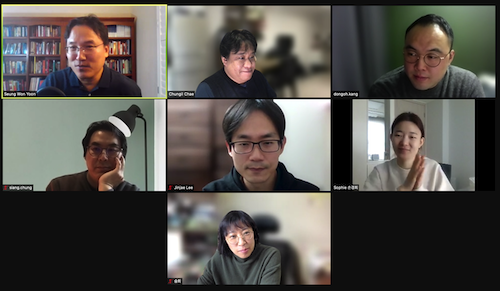
\includegraphics{img/s1/1.png}

\hypertarget{session1---chapter1-2-1}{%
\chapter{Session1 - Chapter1 \& 2}\label{session1---chapter1-2-1}}

\hypertarget{uxbc1cuxd45cuxc790uxb8cc-1}{%
\section{발표자료}\label{uxbc1cuxd45cuxc790uxb8cc-1}}

\begin{itemize}
\tightlist
\item
  \href{https://www.notion.so/Ch3-4-Describing-Data-Continuous-Vars-f074b5ea4b7849b69c14a65d04f8aeeb}{노션}
\item
  \href{https://drive.google.com/file/d/1EC1y9vQwPwn-uGACFh5XblTW_ENIFtPE/view?usp=sharing}{PDF}
\end{itemize}

\hypertarget{uxc694uxc57d-1}{%
\section{요약}\label{uxc694uxc57d-1}}

\begin{itemize}
\tightlist
\item
  체크인 질문: 지난한주를 다섯글자로 표현하고 그 이유를 설명

  \begin{itemize}
  \tightlist
  \item
    중장기계획, 너무바빳음, 롤러코스터, 지옥과천국, 백신맞은주, 샤이니만세, 휴가후여파, 티끌모아태산, 이럴줄알았(다), 새해엔다들
  \end{itemize}
\item
  챕터요약: 발표자료 참조
\item
  디스커션

  \begin{itemize}
  \tightlist
  \item
    시뮬레이션: R이 없는 데이터를 잘 채워넣어준다
  \item
    Factor - 유용성, 더미코딩
  \item
    랜덤제너레이션에서 시간스템프를 사용
  \item
    마케팅 데이터가 Transformation을 자주하더라 실무적으로 유용할것 같다
  \item
    분포와 샘플링 중요
  \item
    내 업무에서는 어떤 데이터, 어떤 분포의 데이터를 주로?
  \item
    데이터 전처리의 중요성
  \item
    Box-Cox변환 \url{https://m.blog.naver.com/jiehyunkim/220616091027}
  \item
    회원등급과 행동의 상관관계
  \item
    실무에서의 접근 시작점 (이 물건을 어떻게 팔아야 할 것인가)
  \item
    현상은 동일하지만 목적에 따라(산업) 필요한 데이터가 달라짐
  \item
    일본사례 이탈자분석 (2014년) \url{https://gamebiz.jp/news/131227}
  \item
    \href{https://www.r-graph-gallery.com/}{R graph gallery}
  \item
    \href{https://www.python-graph-gallery.com/}{Python graph gallery}
  \item
    \href{https://plotly.com/r/sunburst-charts/}{Sunburst chart}
  \end{itemize}
\end{itemize}

\hypertarget{uxd604uxc7a5uxc0acuxc9c4-1}{%
\section{현장사진}\label{uxd604uxc7a5uxc0acuxc9c4-1}}

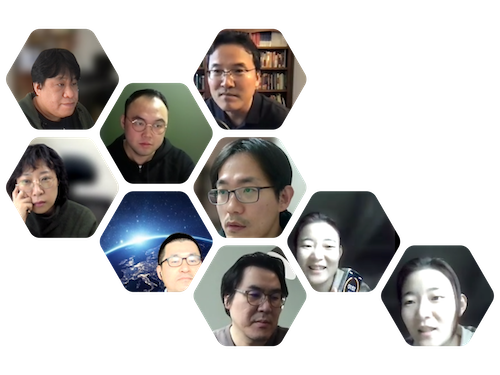
\includegraphics{img/s2/3.png}

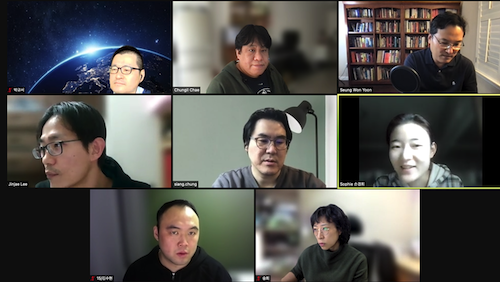
\includegraphics{img/s2/1.png}

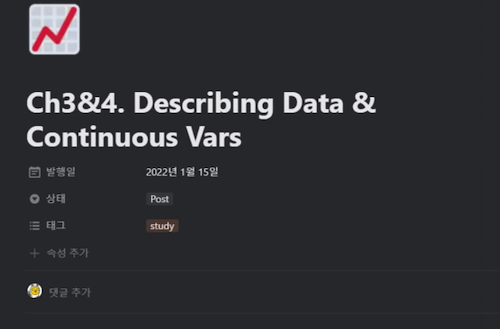
\includegraphics{img/s2/2.png}

\printbibliography

\end{document}
